% me=0 student solutions (ps file), me=1 - my solutions (sol file),
% me=2 - assignment (hw file)
\def\me{0} \def\num{11} %homework number

\def\due{Thursday, 5 pm on December 5} %due date

\def\course{CSCI-GA.1170-001/002 Fundamental Algorithms} 
%course name, changed only once

% **** INSERT YOUR NAME HERE ****
\def\name{jingshuai jiang}

% **** INSERT YOUR NETID HERE ****
\def\netid{jj2903}

% **** INSERT NETIDs OF YOUR COLLABORATORS HERE ****
\def\collabs{NetID1, NetID2}


\iffalse

INSTRUCTIONS: replace # by the homework number.  (if this is not
ps#.tex, use the right file name)

Clip out the ********* INSERT HERE ********* bits below and insert
appropriate LaTeX code.  There is a section below for student macros.
It is not recommended to change any other parts of the code.


\fi
%

\documentclass[11pt]{article}


% ==== Packages ====
\usepackage{amsfonts,amsmath}
\usepackage{latexsym}
\usepackage{fullpage}
\usepackage{graphicx}
\usepackage{tikz}
\usepackage[bottom]{footmisc}


% \setlength{\oddsidemargin}{.0in} \setlength{\evensidemargin}{.0in}
% \setlength{\textwidth}{6.5in} \setlength{\topmargin}{-0.4in}
\setlength{\footskip}{1in} \setlength{\textheight}{8.5in}

\newcommand{\handout}[5]{
\renewcommand{\thepage}{#1, Page \arabic{page}}
  \noindent
  \begin{center}
    \framebox{ \vbox{ \hbox to 5.78in { {\bf \course} \hfill #2 }
        \vspace{4mm} \hbox to 5.78in { {\Large \hfill #5 \hfill} }
        \vspace{2mm} \hbox to 5.78in { {\it #3 \hfill #4} }
        \ifnum\me=0
        \vspace{2mm} \hbox to 5.78in { {\it Collaborators: \collabs
            \hfill} }
        \fi
      } }
  \end{center}
  \vspace*{4mm}
}

\newcounter{pppp}
\newcommand{\prob}{\arabic{pppp}} %problem number
\newcommand{\increase}{\addtocounter{pppp}{1}} %problem number

% Arguments: Title, Number of Points
\newcommand{\newproblem}[2]{
  \ifnum\me=0
    \ifnum\prob>0 \newpage \fi
    \increase
    \setcounter{page}{1}
    \handout{\name{} (\netid), Homework \num, Problem \arabic{pppp}}
    {\today}{Name: \name{} (\netid)}{Due: \due}
    {Solutions to Problem \prob\ of Homework \num\ (#2)}
  \else
    \increase
    \section*{Problem \num-\prob~(#1) \hfill {#2}}
  \fi
}

% \newcommand{\newproblem}[2]{\increase
% \section*{Problem \num-\prob~(#1) \hfill {#2}}
% }

\def\squarebox#1{\hbox to #1{\hfill\vbox to #1{\vfill}}}
\def\qed{\hspace*{\fill}
  \vbox{\hrule\hbox{\vrule\squarebox{.667em}\vrule}\hrule}}
\newenvironment{solution}{\begin{trivlist}\item[]{\bf Solution:}}
  {\qed \end{trivlist}}
\newenvironment{solsketch}{\begin{trivlist}\item[]{\bf Solution
      Sketch:}} {\qed \end{trivlist}}
\newenvironment{code}{\begin{tabbing}
    12345\=12345\=12345\=12345\=12345\=12345\=12345\=12345\= \kill }
  {\end{tabbing}}

%\newcommand{\eqref}[1]{Equation~(\ref{eq:#1})}

\newcommand{\hint}[1]{({\bf Hint}: {#1})}
% Put more macros here, as needed.
\newcommand{\room}{\medskip\ni}
\newcommand{\brak}[1]{\langle #1 \rangle}
\newcommand{\bit}[1]{\{0,1\}^{#1}}
\newcommand{\zo}{\{0,1\}}
\newcommand{\C}{{\cal C}}

\newcommand{\nin}{\not\in}
\newcommand{\set}[1]{\{#1\}}
\renewcommand{\ni}{\noindent}
\renewcommand{\gets}{\leftarrow}
\renewcommand{\to}{\rightarrow}
\newcommand{\assign}{:=}

\newcommand{\AND}{\wedge}
\newcommand{\OR}{\vee}

\newcommand{\For}{\mbox{\bf for }}
\newcommand{\To}{\mbox{\bf to }}
\newcommand{\DownTo}{\mbox{\bf downto }}
\newcommand{\Do}{\mbox{\bf do }}
\newcommand{\If}{\mbox{\bf if }}
\newcommand{\Then}{\mbox{\bf then }}
\newcommand{\Else}{\mbox{\bf else }}
\newcommand{\While}{\mbox{\bf while }}
\newcommand{\Repeat}{\mbox{\bf repeat }}
\newcommand{\Until}{\mbox{\bf until }}
\newcommand{\Return}{\mbox{\bf return }}
\newcommand{\Halt}{\mbox{\bf halt }}
\newcommand{\Swap}{\mbox{\bf swap }}
\newcommand{\Ex}[2]{\textrm{exchange } #1 \textrm{ with } #2}
\newcommand{\Nil}{\mbox{\bf nil }}
\newcommand{\False}[0]{\mathsf{False}}
\newcommand{\True}[0]{\mathsf{True}}

\begin{document}

\ifnum\me=0

% Collaborators (on a per task basis):
%
% Task 1: *********** INSERT COLLABORATORS HERE *********** 
% Task 2: *********** INSERT COLLABORATORS HERE *********** 
% etc.
%

\fi

\ifnum\me=1

\handout{PS \num}{\today}{Lecturer: Yevgeniy Dodis}{Due: \due}
{Solution {\em Sketches} to Problem Set \num}

\fi

\ifnum\me=2

\handout{PS \num}{\today}{Lecturer: Yevgeniy Dodis}{Due: \due}{Problem
  Set \num}

\fi


\newproblem{Inequalities and Consistencies}{9+8 points}

You are given a set $V$ of $n$ variables, $\{x_1,\ldots,x_n\}$
and a set $C$ of $m$ strict inequalities, i.e, of the form $x_i<x_j$. The set
$C$ of inequalities is called \emph{consistent} over
the set of positive integers $\mathbb{Z}^+$ iff there
exists an assignment of positive integer values in
such a way that it satisfies all the inequalities. For example,
$x_1< x_2, x_2<x_3,x_3< x_1$ is not consistent but $x_1<x_2,x_2<x_3$ is consistent. 
The goal
of this question is to formulate an algorithm to determine
whether $C$ is consistent or not and then assign minimum possible value 
that satisfies these constraints over the set of positive integers.

\begin{enumerate}
	\item[(a)](4 points) Give an $O(m+n)$ algorithm to determine whether
	the set $C$ of inequalities is consistent. State 
	precisely the asymptotic running time of your algorithm 
	in terms of $n$ and $m$. Argue the correctness of your algorithm. 
	\hint{Represent this as a graph
	and use one of the graph algorithms. You are not allowed
	to assign weights to edges.}
	\ifnum\me<2
\begin{solution}   
In this problem, we should think of these variables as vertices of graph and these inequalities as edges. If this set C of inequalities is consistent, then our graph should be acyclic. Then we can turn this problem into a graph problem, wihch determines whether there is a cycle in this graph.\\[10pt]
\begin{code}
	1 {\sc DFSconsistent}$(G)$\\
	2 \> \For each $u$ in $V$ \\
	3 \> \> $u.color = white$\\
	4 \> \> $u.\pi = NIL$\\
	5 \> \For each $u$ in $V$ \\
	6 \> \>if $u.color == white$\\
	7 \> \> \> if IsConsistent(G,u)==false, return false\\
	8 \> return True\\
\end{code}
\begin{code}
	1 {\sc IsConsistent}$(G,u)$\\
	2 \> u.color = GRAY \\
	3 \> \For each $v$ in G.adj[u]\\
	3 \> \> \If v.color == GRAY, return false;\\
	4\> \> \If v.color ==white\\
	5\>\>\> \If IsConsistent(G,v)==false, return false;\\
	7\> u.color = black\\
	8\> return true;\\
\end{code}
In this code i am using an dfs search. If we met a back edge then there is a cycle in this graph. That means it is not consistent. By using the three color, we can know whether we have a backedge by pending on whether we met a gray node.
The running time will be O(m+n).
\end{solution}
	\fi
	\item[(b)](5 points) Give an $O(m+n)$ algorithm {\sc Assign-Value} to find
	the minimum possible solution over the set of \emph{positive}
	integers, assuming $C$ is consistent. Briefly argue the correctness
	and the runtime of your algorithm. \hint{Use topological sort.}
	\begin{code}
		1 {\sc Driver}$(G)$\\
		2 \> \For $v$ in $V$ \\
		3 \> \> $v.value=1$\\
		3 \> {\sc Assign-Value}$(G)$\\
		\vspace{1mm}\\
			\end{code}
	\ifnum\me<2
\begin{solution}
	\begin{code}
		1 {\sc reverse-topological-sort}$(G)$\\
		2 \> call DFS(G) to computer finishing time v.f for each vertex v\\
		3 \> as each vertex is finished, insert it onto the front of a linked list\\
		4 \> reverse this linked list\\
	\end{code}   
	\begin{code}
		1 {\sc Assign-Value}$(G)$\\
		2 \> list = reverse-topological-sort(G)\\		
		3 \>for node from head to tail\\ 
		4 \>\> if node.adj is not NIL,\Then v.value = $\max_{u\in adj[v]} {u.value}+1$\\
	\end{code}
	We turn this problem into a graph problem. The symbol $x1<x2$ means there is an edge from $x2$ to $x1$. And we use topological sort to determine which node finish first. \\[10pt]
	\textbf{1:} if the node has no adjcent list, which means it has no constraints on its value. Then we just need to assign the samllest value to it.\\[10pt]
	\textbf{2:} If the node does have adjcent list, we need to check all its neighbours and since it should be bigger than its neighbours . Then we just need to take the maximum value of all its neighbours and add 1 to this maximum value.
	Since we have used the topological sort, we have already calculated the value of this nodes neighbours. \\[10pt]
	The runtime of this algorithm will be the same as topological sort, which is O(V+E) = O(m+n).
\end{solution}
	\fi
\end{enumerate}
While we spoke about strict inequalities, we can also look at weak inequalities.
These typically involve the operators $\leq,\geq$. Indeed, a strict equality 
of the form $x_i<x_j$ can be rewritten as $x_i\leq x_j-1$ provided $x_i,x_j$
are over the set of integers. Therefore, one can look at the generalized
case where $C$ contains inequalities of the form $x_i\leq x_j-c$ where $c\geq 0$.
\begin{enumerate}
	\item[(c)] \textbf{(Extra Credit)} (8 points) Consider the above
	generalization where the set $C$ contains 
	inequalities of the form $x_i\leq x_j-c$ where $c\geq 0$. Design an $O(m+n)$
	algorithm  to determine if the set $C$ is 
	consistent. Further, design an $O(m+n)$ algorithm that
	provides the least possible satisfying assignment, provided $C$ is consistent.
	Argue correctness of your algorithms. You may describe the algorithm in words.
	\hint{Consider adding edge weights. Use the SCC algorithm.}
	\ifnum\me<2
\begin{solution}  
	\textbf{Problem transformation}:
	The variables will be viewed as vertices of graph. The weak inequalities will be viewed as edges among these vertices. And the constant c will be viewed as the weight of these edges.\\[10pt]
	We use these rules to build a graph G\\[10pt]
	\textbf{Consistency}:
	First we run DFS on this newly built graph.\\[10pt]
	During the process of DFS, when we traverse each node v in the adjlist of vertice u, if this v.color is gray, then we will know there is a cycle in this graph. If not all the weights on these edge are equal to zero. Then this graph is not consistent. Otherwise we continue our DFS. If there is no this unusual cycle then it is consistent\\[10pt]
	
	\textbf{Assign-Value}:
	
\end{solution}
	\fi
	\end{enumerate}


\newproblem{Cost of a Switch}{10 Points}

Let us assume that you are given a directed graph $G=(V,E)$. Each $v\in V$  
is assigned $v.w\in\{0,1\}$. Let the cost of a path $v_1,\ldots,v_k$ 
be the number of times the path switches in weights. More concretely, 
$\sum_{i=1}^{k-1} \vert v_i.w-v_{i+1}.w\vert$. Note that
some of these nodes might be the same, i.e, the path can revisit nodes already visited.
Consider the following graph:


\begin{center}


\tikzset{every picture/.style={line width=0.75pt}} %set default line width to 0.75pt        

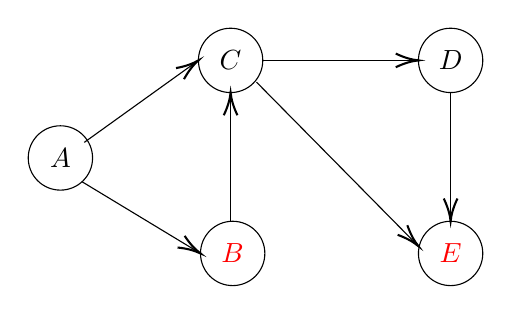
\begin{tikzpicture}[x=0.75pt,y=0.75pt,yscale=-1,xscale=1]
%uncomment if require: \path (0,300); %set diagram left start at 0, and has height of 300

%Shape: Circle [id:dp7030373692721936] 
\draw   (138,64.5) .. controls (138,55.94) and (144.94,49) .. (153.5,49) .. controls (162.06,49) and (169,55.94) .. (169,64.5) .. controls (169,73.06) and (162.06,80) .. (153.5,80) .. controls (144.94,80) and (138,73.06) .. (138,64.5) -- cycle ;
%Shape: Circle [id:dp055972558634265424] 
\draw   (139,157.5) .. controls (139,148.94) and (145.94,142) .. (154.5,142) .. controls (163.06,142) and (170,148.94) .. (170,157.5) .. controls (170,166.06) and (163.06,173) .. (154.5,173) .. controls (145.94,173) and (139,166.06) .. (139,157.5) -- cycle ;
%Straight Lines [id:da8719020208792478] 
\draw    (153.5,82) -- (153.5,142) ;

\draw [shift={(153.5,80)}, rotate = 90] [color={rgb, 255:red, 0; green, 0; blue, 0 }  ][line width=0.75]    (10.93,-3.29) .. controls (6.95,-1.4) and (3.31,-0.3) .. (0,0) .. controls (3.31,0.3) and (6.95,1.4) .. (10.93,3.29)   ;
%Shape: Circle [id:dp04166645672311908] 
\draw   (56,111.5) .. controls (56,102.94) and (62.94,96) .. (71.5,96) .. controls (80.06,96) and (87,102.94) .. (87,111.5) .. controls (87,120.06) and (80.06,127) .. (71.5,127) .. controls (62.94,127) and (56,120.06) .. (56,111.5) -- cycle ;
%Straight Lines [id:da5517052364618521] 
\draw    (83,104) -- (136.38,65.67) ;
\draw [shift={(138,64.5)}, rotate = 504.31] [color={rgb, 255:red, 0; green, 0; blue, 0 }  ][line width=0.75]    (10.93,-3.29) .. controls (6.95,-1.4) and (3.31,-0.3) .. (0,0) .. controls (3.31,0.3) and (6.95,1.4) .. (10.93,3.29)   ;

%Straight Lines [id:da8449783032969879] 
\draw    (82,123) -- (137.29,156.46) ;
\draw [shift={(139,157.5)}, rotate = 211.18] [color={rgb, 255:red, 0; green, 0; blue, 0 }  ][line width=0.75]    (10.93,-3.29) .. controls (6.95,-1.4) and (3.31,-0.3) .. (0,0) .. controls (3.31,0.3) and (6.95,1.4) .. (10.93,3.29)   ;

%Shape: Circle [id:dp9327114180599945] 
\draw   (244,64.5) .. controls (244,55.94) and (250.94,49) .. (259.5,49) .. controls (268.06,49) and (275,55.94) .. (275,64.5) .. controls (275,73.06) and (268.06,80) .. (259.5,80) .. controls (250.94,80) and (244,73.06) .. (244,64.5) -- cycle ;

%Shape: Circle [id:dp6730949389302344] 
\draw   (244,157.5) .. controls (244,148.94) and (250.94,142) .. (259.5,142) .. controls (268.06,142) and (275,148.94) .. (275,157.5) .. controls (275,166.06) and (268.06,173) .. (259.5,173) .. controls (250.94,173) and (244,166.06) .. (244,157.5) -- cycle ;
%Straight Lines [id:da1273886918860302] 
\draw    (169,64.5) -- (242,64.5) ;
\draw [shift={(244,64.5)}, rotate = 180] [color={rgb, 255:red, 0; green, 0; blue, 0 }  ][line width=0.75]    (10.93,-3.29) .. controls (6.95,-1.4) and (3.31,-0.3) .. (0,0) .. controls (3.31,0.3) and (6.95,1.4) .. (10.93,3.29)   ;

%Straight Lines [id:da9834334340813603] 
\draw    (259.5,80) -- (259.5,140) ;
\draw [shift={(259.5,142)}, rotate = 270] [color={rgb, 255:red, 0; green, 0; blue, 0 }  ][line width=0.75]    (10.93,-3.29) .. controls (6.95,-1.4) and (3.31,-0.3) .. (0,0) .. controls (3.31,0.3) and (6.95,1.4) .. (10.93,3.29)   ;

%Straight Lines [id:da9779391705425159] 
\draw    (242.59,152.58) -- (166,75) ;

\draw [shift={(244,154)}, rotate = 225.36] [color={rgb, 255:red, 0; green, 0; blue, 0 }  ][line width=0.75]    (10.93,-3.29) .. controls (6.95,-1.4) and (3.31,-0.3) .. (0,0) .. controls (3.31,0.3) and (6.95,1.4) .. (10.93,3.29)   ;

% Text Node
\draw (153.5,64.5) node   {$C$};
% Text Node
\draw (154.5,157.5) node   {{\color{red}$B$}};
% Text Node
\draw (71.5,111.5) node   {$A$};
% Text Node
\draw (259.5,64.5) node   {$D$};
% Text Node
\draw (259.5,157.5) node    {{\color{red}$E$}};


\end{tikzpicture}

\end{center}

Let the nodes labeled in red have a weight 1. Therefore, $A.w=C.w=D.w=0$ and $B.w=E.w=1$.
The path $A\rightarrow C\rightarrow D\rightarrow {\color{red}E}$ has a cost of 1 while the path 
$A\rightarrow{\color{red}B}\rightarrow C\rightarrow D\rightarrow  {\color{red}E}$ has a cost of 2. 

\begin{enumerate}
	\item [(a)] (5 points) Design an algorithm that takes as input an \emph{acyclic} graph $G=(V,E)$
	and returns the maximum cost of a path in $G$. This algorithm should run
	in time $O(|V|+|E|)$. Assume that $G$ is represented as an adjacency list. Briefly
	argue correctness of the algorithm.
	\hint{Begin by using an algorithm we covered in class. 
	Then, define $M[v]$ to be the maximum cost of a path starting at $v$. Use a simple
	dynamic programming idea to construct this array $M$.}
	\ifnum\me<2
\begin{solution}   
	\begin{code}
		1 {\sc maximum-cost}$(G)$\\
		2 \> call DFS(G) to computer finishing time v.f for each vertex v\\
		3 \> as each vertex is finished, insert it onto the front of a linked list\\
		4 \> from vertices v from tail to head\\ 
		5 \> \> \If v has no adjcent vertices,then M[v] = 0\\
		6\>\>\Else M[v] = $\max_{u\in v.adj}\left\{M[u]+|v.w-u.w|\right\}$\\
		7 \> return the maximum value of all M\\
	\end{code}
	Firstly we use topological sort to sort this whole graph. Then from tail to head we construct the array M. If the vertice v has no adjcent veritces, then this v must be end to a path. Then the maximum cost of a path
	starting at this end point is 0. If this vertice v has some adjcent vertices, we will choose the maximum cost among its all adjcent veritces. Since we are using topological sort. Then the maximum cost of a vertice's adjcent vertice 
	must be calculated before this vertice. After that we just need to return the maximum value among all the M[V].\\[10pt]
	The runtime of this algorithm will be $O(|V|+|E|)$.

\end{solution}
	\fi
	\item[(b)] (5 points) Now generalize your algorithm to solve this problem
	on any {\em arbitrary} graph. Justify the correctness of your algorithm. \hint{Use another algorithm from class to begin.}
	\ifnum\me<2
\begin{solution}  
	\begin{code}
		1 {\sc generalization}$(G)$\\
		2 \> calculate the strongly connected parts(scc) of this graph G\\
		3 \> \If any part of these scc has both a cycle and weight variation in this cycle,\Then \Return $\infty$\\
		4 \> \Else think of the scc as a vertice, the weight of this vertice should be the same\\ with the vertices inside this scc\\ 
		5 \> \> use the algorithm in part (a) to calculate the maximum cost of this newly built graph\\
		6 \>\> \Return the maximum of M\\
	\end{code}
	\textbf{Correctness}: It is obvious, if a graph contains a cycle and contains weight variation in this cycle, the final cost should be infty. Because the maximum path should contain this infty loop of this cycle.\\[10pt]
	If these strongly connected parts do not have weight variation in the cycle. Then it is easy too. We will think of this part to be a single vertice, with its weight equal to the weight of vertices inside this part.
	Then this problem has been turned into the same problem in part a. Then we can just use the algorithm in part a to solve it. 
\end{solution}
	\fi
\end{enumerate}
\newproblem{Faster Minimum Spanning Trees}{7 points}
For purposes of this question we have a connected, undirected graph $G=(V,E)$ such
that $|E|=m,|V|=n$. Each edge has an assigned weight. 
\noindent
\begin{itemize}

\item[(a)] (3 points) Assume that all edge weights are equal to the same number $w$. Design the fastest algorithm you can to compute the MST of $G$. Argue the correctness of the algorithm and state its run-time. Is it faster than the standard $O(m + n\log n)$ run-time of Prim?

\ifnum\me<2
\begin{solution}   
	\begin{code}
		1\> for each v in G.v \\
		2\>\> $v.\pi = NIL$ and add v to set C\\
		3\>add startpoint s into Q and remove s from C\\
		4 \>while Q is not empty\\
		5\>\> u = Q.dequeue()\\
		6\>\> for each v in u.adjlist\\
		7\>\>\> if v is in C\\
		8\>\>\>\>Remove v from C\\ 
		9\>\>\>\>and add v to Q\\
		10\>\>\>\>$v.\pi = u$\\
		\end{code}
	This code is actually using a variate of BFS. Since all the edges have the same weight, we do not need to think about how to minimize the whole weight. We just need to add all nodes into our tree for one time.\\[10pt]
	Before we start, we built a set of C, which is a copy of all the nodes in G. \\[10pt]
	Then We start from the startpoint s. Firstly we will remove s from C. And search its adjcent list. If the neighbour is still in C, then we add it to the queue and remove it from C and keep searching.\\[10pt]
	In this algorithm each node will be add into the queue for only one time. And the edge will be searching for one time. Then the total runtime is $O(m+n)$.\\[10pt]
	It is faster than the standard $O(m+nlogn)$
\end{solution}
\fi

\item[(b)] (4 points) Now assume the all the edge weights are equal to $w$, except for a single edge $e'=(u',v')$ whose weight is $w'$ (note, $w'$ might be either larger or smaller than $w$). Show how to modify your solution in part (a) to compute the MST of $G$. What is the running time of your algorithm and how does it compare to the run-time you obtained in part (a) (or standard Prim)? \hint{Consider different cases, first based on 
whether $e'$ is needed in the MST or not. Then, based on if $w'>w$ or not.}

\ifnum\me<2
\begin{solution}   
Firstly we should decide whether we need this edge.
By scanning all the edges we find this special edge $e'$. If any of the two vertices connected by this edge can only be reached by this edge, then this edge is obviously needed no matter whewher it is bigger than others.
Then we just need to ran the algorithm in Part 1.\\[10pt]

Secondly if this edges is not a necessary, then we should compare its weight $w'$ to $w$ if it is bigger than the $w$, then we just delete this edge from both of its edge's adjcentlist. And run the algorithm from part1.\\[10pt]
Thirdly if the weight of this edges  $w'$ is smaller than $w$. Then we choose one of its vertices to be the start point and use the part1 solution.\\[10pt]
\textbf{Runtime}:In our solution, the process of find this special edge takes time $O(|E|)$, and decide whether we need it takes $O(1)$ time. 
The process of deleting this bigger edge from the adjcentlist takes the worst time $O(|E|)$.
And the process of part 1 takes time $O(|E|+|V|)$
The total runtime will be $O(3|E|+|V|)$ = $O(|E|+|V|)$. It is better than standard Prim. But it should be worse than algorithm in part 1 because part1 is one part in part2. But in asymptotic meaning they are in the same level.
\end{solution}
\fi
\end{itemize}
\newproblem{Extra Credit: Bounded Weight MST}{14 points}
For purposes of this question we have a connected, undirected graph $G=(V,E)$ such
that $|E|=m,|V|=n$. Assume all edge weights in $G$ are integers from $1$ to $w$.

\begin{itemize}

\item[(a)] (3 points) Show how to modify Prim's algorithm to achieve running time $O(m+nw)$. Hence, if $w=O(1)$, you get optimal  time $O(m+n)$.  Recall that Prim's algorithm makes $n$ {\sc Extract-Min} operation and 
$m$ {\sc Decrease-Key} operation. Clearly, explain how your modification would 
implement {\sc Extract-Min} and {\sc Decrease-Key} and what the runtime is.  \hint{Priority queues are typically
implemented using a heap. However, in this example use a doubly linked 
list as the underlying data structure. How many such lists do you need? }

\ifnum\me<2
\begin{solution}   
In this problem we will have w doubly linked list for values between 1 to w. The ith list will store nodes whose value is i.\\[10pt]
\textbf{For ExtractMin:} We check if the 1st list is empty. If not,extract one from the list. If it is empty, we check the 2nd list. Then untill the wth list. This runtime will be $O(w)$\\[10pt]
\textbf{For DecreaseKey:} We remove the node from its orginal list and add it to its new list.\\[10pt]
\textbf{Runtime:} The ExtractMin takes time $O(w)$, the DecreaseKey takes time $O(1)$, Since the whole time of prim is $O(n \cdot T_{ExtractMin}+m \cdot T_{DecreaseKey})$, then it is $O(m+nw)$.
\end{solution}
\fi
\item[(b)] (6 points) Show how to modify the above algorithm further to achieve a running time of $O(m+n\log w)$. Clearly, explain how your modification would 
implement {\sc Extract-Min} and {\sc Decrease-Key} and what the runtime is. \hint{
Implement the priority queue using the linked lists but by storing them in an efficient fashion. You may find it useful to employ a Fibonacci Heap in a black box fashion. You may use the Wikipedia page of Fibonacci Heap to retrieve the running time of the various operations.}
\ifnum\me<2
\begin{solution}   
	In this problem we will have w  linked list for values between 1 to w. The ith list will store nodes whose value is i. And the head node of these w list will be store in a Fibonacci heap\\[10pt]
	\textbf{For ExtractMin:} We use the heap to do the extract thing. Extract the minimum value in a W nodes heap takes time $O(logw)$. \\[10pt]
	\textbf{For DecreaseKey:} We remove the node from its orginal list and add it to its new list. \\[10pt]
	\textbf{Runtime:} The ExtractMin takes time $O(logw)$, the DecreaseKey takes time $O(1)$, Since the whole time of prim is $O(n \cdot T_{ExtractMin}+m \cdot T_{DecreaseKey})$, then it is $O(m+nlogw)$.
\end{solution}
\fi

\end{itemize}
Recall that the runtime of Kruskal's Algorithm is $O(m\log m+ m\cdot T_{find}+n\cdot T_{union})$.
	There are set-disjoint data structures, as discussed in class, where $T_{find}=T_{union}=\alpha(n)$
	where $\alpha(n)$ is a certain function much smaller than $\log n$. 
\begin{itemize}
\item[(c)] (3 points) Now assume $w=n$, so that the previous solution in part (a) is no longer faster than standard. 
	Show how to modify Kruskal's algorithm, so that your modified algorithm now takes time $O(m\cdot \alpha(n))$, instead of $O(m\log n)$. 
\ifnum\me<2
\begin{solution}   

\end{solution}
\fi

\item[(d)](2 points) What is the largest $w$, as a function of $\alpha(n)$, for which you can still maintain the run-time in part $c$? 

\ifnum\me<2
\begin{solution}   

\end{solution}
\fi

\end{itemize}


\end{document}


